\chapter{Fractional-Order Differential Equations}
\label{ch:diffeq}

\begin{example}
  Determine the solution to
  \begin{equation*}
    \frac{\d^{\frac{1}{2}}x}{\d t^{\frac{1}{2}}}(t) + a x(t) = f(t)
  \end{equation*}
  where we use the Riemann-Liouville fractional derivative, or
  \begin{equation}
    \tensor*[^{RL}]{\D}{^{\frac{1}{2}}} x(t) + a x(t) = f(t).
    \label{eq:fracdiffeqex1}
  \end{equation}
Computing the Laplace transform of each side of the equation gives
\begin{equation*}
  s^\frac{1}{2} X(s) - \left[ \tensor*[]{\D}{^{-\frac{1}{2}}} x(t) \right]_{t=0} + a X(s) = F(s).
\end{equation*}
For the time being, let us assume that the initial condition term is not zero, and call it $c$. Solving for $X(s)$ gives
\begin{equation*}
  X(s) = \frac{c}{\sqrt{s} + a} + \frac{F(s)}{\sqrt{s} + a}.
\end{equation*}

If $f(t) = 0$ and $c = 1$, then
\begin{equation*}
  X(s) = \frac{1}{\sqrt{s}+a}
\end{equation*}
and the Laplace transform table gives that 
\begin{equation*}
  x(t) = \frac{1}{\sqrt{t}} \E_{\frac{1}{2},\frac{1}{2}}\left( a \sqrt{t} \right). 
\end{equation*}
The solution to this equation is illustrated in Figure~\ref{fig:fracdiffeqex1a}. Note for increasing $a$ the solution decays more rapidly. A graph of $x(t) = \e^{-2 t}$ is also shown for comparison.

\begin{figure}
  \centering
  \subimport{figs/}{fracdiffeqex1a}
  \caption{Solutions to Equation~\ref{eq:fracdiffeqex1} for various $a = 1/2$ (blue), $a=1$ (red), $a=3.2$ gold and $a=2$ (purple) and $f(t)=0$ and $x(t) = e^{-2 t}$ (green) for comparison.}
  \label{fig:fracdiffeqex1a}
\end{figure}

Now, assume that $f(t) = 1$, so that $F(s) = 1/s$, in which case
\begin{equation}
  X(s) = \frac{1}{\sqrt{s} + a} + \frac{1}{s \left( \sqrt{s} + a \right)}.
\end{equation}
From Table~\ref{tab:ltpairs}, for the second term, we need that $\alpha = 1/2$ and in order to get the other $s$ term in the denominator, we need $\beta - \alpha = 1$, so $\beta = 3/2$, which gives
\begin{equation*}
  x(t) = \frac{1}{\sqrt{t}} \E_{\frac{1}{2},\frac{1}{2}} \left( a \sqrt{t} \right) + \sqrt{t} \E_{\frac{1}{2},\frac{3}{2}} \left( a \sqrt{t} \right).
\end{equation*}

Figure~\ref{fig:fracdiffeqex1b} illustrates the solutions when $c=0$, \ie, it is the``step response'' portion of the solution. Figure~\ref{fig:fracdiffeqex1c} illustrates the full solution including the term with $c=1$.

\begin{figure}
  \centering
  \subimport{figs/}{fracdiffeqex1b}
  \caption{Solutions to Equation~\ref{eq:fracdiffeqex1} for various $a = 1/2$ (blue), $a=1$ (red), $a=3.2$ gold and $a=2$ (purple), $f(t)=1$ and $c=0$  and $x(t) = 1 - e^{-2 t}$ (green) for comparison.}
  \label{fig:fracdiffeqex1b}
\end{figure}

\begin{figure}
  \centering
  \subimport{figs/}{fracdiffeqex1c}
\caption{Solutions to Equation~\ref{eq:fracdiffeqex1} for various $a = 1/2$ (blue), $a=1$ (red), $a=3.2$ gold and $a=2$ (purple), $f(t)=1$ and $c=1$.}
  \label{fig:fracdiffeqex1c}
\end{figure}
\end{example}

\begin{example}
  As a second example, consider a mass attached to a wall and subjected to a force as illustrated in Figure~\ref{fig:masswall}. We will consider the attachment to the wall as having some sort of mechanical impendence, which could be a spring, or a damper or perhaps a fractional-order type network such as the $1/2$-order tree network of springs and dampers considered earlier in Section~\ref{sec:introexamples}. The top part of the figure illustrates the half-order connection, and the bottom part represents the more general situation where the order of the relationship between the force resisting the motion and the displacement is of order $\gamma$.

  \begin{figure}
    \centering
    \psfrag{f}{$f$}
    \psfrag{m}{$m$}
    \psfrag{x1}{$x$}
    \psfrag{q}{$Q(s^\gamma)$}
    \psfrag{k}{$k$}
    \psfrag{b}{$b$}
    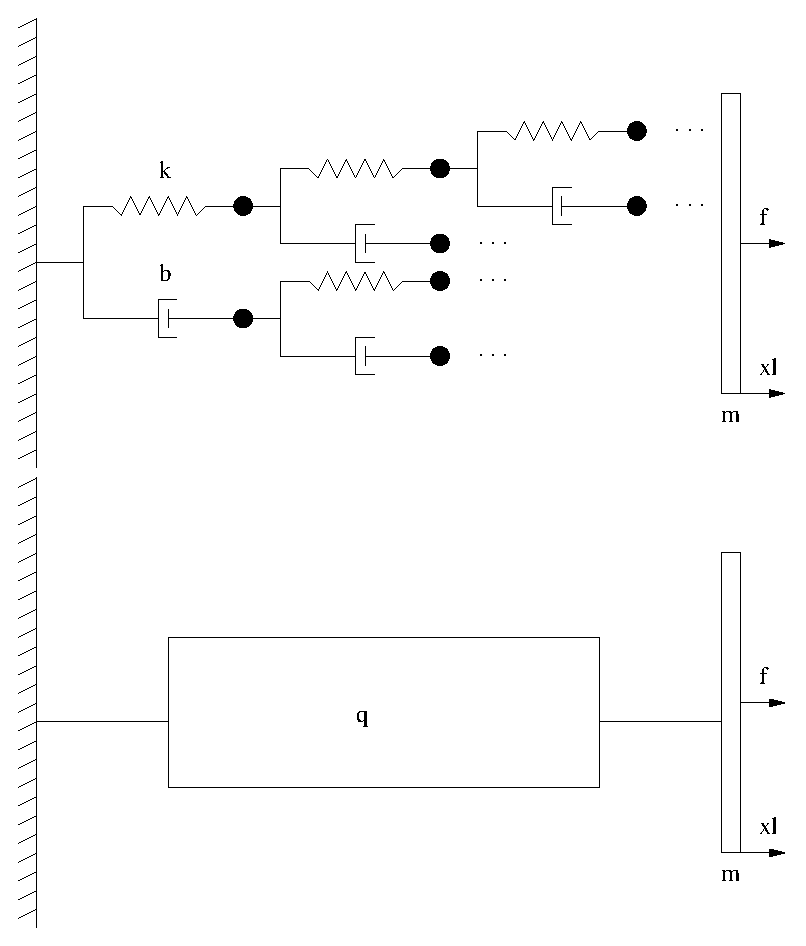
\includegraphics[width=3.5in]{figs/structurewall}
    \caption{Mass attached to a wall.}
    \label{fig:masswall}
  \end{figure}

  Newton's law on the mass gives
  \begin{equation*}
    m \frac{\d^2 x}{\d t^2}(t) + q \frac{\d^\gamma x}{\d t^\gamma}(t) = f(t).
  \end{equation*}
  In the case where the connection is a spring, we would use $q = k$ and $\gamma = 0$, and when it is a damper, we would use $q = b$ and $\gamma = 1$. Divide both sides by $m$, let $f(t)$ be a unit step input, assume zero initial conditions of all orders and take the Laplace transform of both sides, which gives
  \begin{equation}
    X(s) = \frac{1}{s \left(s^2 + \frac{q}{m} s^\gamma \right)} = \frac{1}{s^{\gamma + 1} \left( s^{2 - \gamma} + \frac{q}{m} \right) }.
    \label{eq:sw1}
  \end{equation}

  Referring to Table~\ref{tab:ltpairs}, $\alpha =  2 - \gamma$ and $\alpha - \beta = - \left( \gamma + 1 \right)$, so $\beta = 3$, and the time domain response is
  \begin{equation*}
    x(t) = t^2 \E_{2-\gamma,3}\left(-\frac{q}{m} t^{2 - \gamma} \right).
  \end{equation*}
  
  To validate this, let us plot the solution for $\gamma = 0$, which would correspond to the connection being a spring, in which case we expect a purly oscillatory response. Additionally, if we increase $q/m$ we expect a higher frequency response. Both of these attributes of the solution are illustrated in Figure~\ref{fig:structurewall1}. In the case where $\gamma=1$, the connection to the wall is a damper, in which case we would expect the steady-state solution to be a constant velocity where the damper force and applied force are in equilibrium. This case is illustrated in Figure~\ref{fig:structurewall2}. 

  \begin{figure}
    \centering
    \subimport{figs/}{structurewall1}
    \caption{Solution to Equation~\ref{eq:sw1} in the case where $\gamma=0$, corresponding to a spring element connecting the mass to the wall. The blue curve is for $q/m=1$ and the red curve is for $q/m=2$.}
    \label{fig:structurewall1}
  \end{figure}

  \begin{figure}
    \centering
    \subimport{figs/}{structurewall2}
    \caption{Solution to Equation~\ref{eq:sw1} in the case where $\gamma=1$, corresponding to a damper element connecting the mass to the wall.}
    \label{fig:structurewall2}
  \end{figure}

  Finally, the solutions for $\gamma \in \left\{ 0, 0.25, 0.5, 0.75, 1, 1.25, 1.5, 1.75 \right\}$ are illustrated in Figure~\ref{fig:structurewall3}. We will revisit this problem in the next chapter when we consider numerical methods.

 \begin{figure}
    \centering
    \subimport{figs/}{structurewall3}
    \caption{Solution to Equation~\ref{eq:sw1} for $\gamma = 0, 0.25, 0.5, \ldots, 1.75$. }
    \label{fig:structurewall3}
  \end{figure}



\end{example}
